\documentclass[1p]{elsarticle_modified}
%\bibliographystyle{elsarticle-num}

%\usepackage[colorlinks]{hyperref}
%\usepackage{abbrmath_seonhwa} %\Abb, \Ascr, \Acal ,\Abf, \Afrak
\usepackage{amsfonts}
\usepackage{amssymb}
\usepackage{amsmath}
\usepackage{amsthm}
\usepackage{scalefnt}
\usepackage{amsbsy}
\usepackage{kotex}
\usepackage{caption}
\usepackage{subfig}
\usepackage{color}
\usepackage{graphicx}
\usepackage{xcolor} %% white, black, red, green, blue, cyan, magenta, yellow
\usepackage{float}
\usepackage{setspace}
\usepackage{hyperref}

\usepackage{tikz}
\usetikzlibrary{arrows}

\usepackage{multirow}
\usepackage{array} % fixed length table
\usepackage{hhline}

%%%%%%%%%%%%%%%%%%%%%
\makeatletter
\renewcommand*\env@matrix[1][\arraystretch]{%
	\edef\arraystretch{#1}%
	\hskip -\arraycolsep
	\let\@ifnextchar\new@ifnextchar
	\array{*\c@MaxMatrixCols c}}
\makeatother %https://tex.stackexchange.com/questions/14071/how-can-i-increase-the-line-spacing-in-a-matrix
%%%%%%%%%%%%%%%

\usepackage[normalem]{ulem}

\newcommand{\msout}[1]{\ifmmode\text{\sout{\ensuremath{#1}}}\else\sout{#1}\fi}
%SOURCE: \msout is \stkout macro in https://tex.stackexchange.com/questions/20609/strikeout-in-math-mode

\newcommand{\cancel}[1]{
	\ifmmode
	{\color{red}\msout{#1}}
	\else
	{\color{red}\sout{#1}}
	\fi
}

\newcommand{\add}[1]{
	{\color{blue}\uwave{#1}}
}

\newcommand{\replace}[2]{
	\ifmmode
	{\color{red}\msout{#1}}{\color{blue}\uwave{#2}}
	\else
	{\color{red}\sout{#1}}{\color{blue}\uwave{#2}}
	\fi
}

\newcommand{\Sol}{\mathcal{S}} %segment
\newcommand{\D}{D} %diagram
\newcommand{\A}{\mathcal{A}} %arc


%%%%%%%%%%%%%%%%%%%%%%%%%%%%%5 test

\def\sl{\operatorname{\textup{SL}}(2,\Cbb)}
\def\psl{\operatorname{\textup{PSL}}(2,\Cbb)}
\def\quan{\mkern 1mu \triangleright \mkern 1mu}

\theoremstyle{definition}
\newtheorem{thm}{Theorem}[section]
\newtheorem{prop}[thm]{Proposition}
\newtheorem{lem}[thm]{Lemma}
\newtheorem{ques}[thm]{Question}
\newtheorem{cor}[thm]{Corollary}
\newtheorem{defn}[thm]{Definition}
\newtheorem{exam}[thm]{Example}
\newtheorem{rmk}[thm]{Remark}
\newtheorem{alg}[thm]{Algorithm}

\newcommand{\I}{\sqrt{-1}}
\begin{document}

%\begin{frontmatter}
%
%\title{Boundary parabolic representations of knots up to 8 crossings}
%
%%% Group authors per affiliation:
%\author{Yunhi Cho} 
%\address{Department of Mathematics, University of Seoul, Seoul, Korea}
%\ead{yhcho@uos.ac.kr}
%
%
%\author{Seonhwa Kim} %\fnref{s_kim}}
%\address{Center for Geometry and Physics, Institute for Basic Science, Pohang, 37673, Korea}
%\ead{ryeona17@ibs.re.kr}
%
%\author{Hyuk Kim}
%\address{Department of Mathematical Sciences, Seoul National University, Seoul 08826, Korea}
%\ead{hyukkim@snu.ac.kr}
%
%\author{Seokbeom Yoon}
%\address{Department of Mathematical Sciences, Seoul National University, Seoul, 08826,  Korea}
%\ead{sbyoon15@snu.ac.kr}
%
%\begin{abstract}
%We find all boundary parabolic representation of knots up to 8 crossings.
%
%\end{abstract}
%\begin{keyword}
%    \MSC[2010] 57M25 
%\end{keyword}
%
%\end{frontmatter}

%\linenumbers
%\tableofcontents
%
\newcommand\colored[1]{\textcolor{white}{\rule[-0.35ex]{0.8em}{1.4ex}}\kern-0.8em\color{red} #1}%
%\newcommand\colored[1]{\textcolor{white}{ #1}\kern-2.17ex	\textcolor{white}{ #1}\kern-1.81ex	\textcolor{white}{ #1}\kern-2.15ex\color{red}#1	}

{\Large $\underline{12a_{0417}~(K12a_{0417})}$}

\setlength{\tabcolsep}{10pt}
\renewcommand{\arraystretch}{1.6}
\vspace{1cm}\begin{tabular}{m{100pt}>{\centering\arraybackslash}m{274pt}}
\multirow{5}{120pt}{
	\centering
	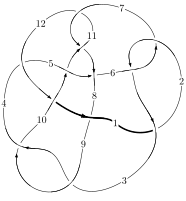
\includegraphics[width=112pt]{../../../GIT/diagram.site/Diagrams/png/1218_12a_0417.png}\\
\ \ \ A knot diagram\footnotemark}&
\allowdisplaybreaks
\textbf{Linearized knot diagam} \\
\cline{2-2}
 &
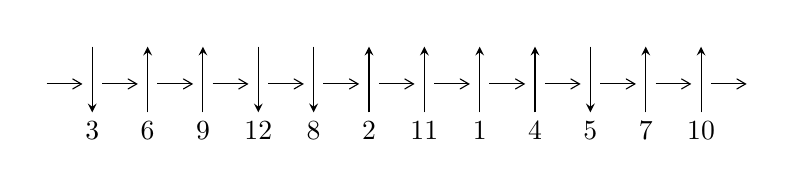
\begin{tikzpicture}[x=20pt, y=17pt]
	% nodes
	\node (C0) at (0, 0) {};
	\node (C1) at (1, 0) {};
	\node (C1U) at (1, +1) {};
	\node (C1D) at (1, -1) {3};

	\node (C2) at (2, 0) {};
	\node (C2U) at (2, +1) {};
	\node (C2D) at (2, -1) {6};

	\node (C3) at (3, 0) {};
	\node (C3U) at (3, +1) {};
	\node (C3D) at (3, -1) {9};

	\node (C4) at (4, 0) {};
	\node (C4U) at (4, +1) {};
	\node (C4D) at (4, -1) {12};

	\node (C5) at (5, 0) {};
	\node (C5U) at (5, +1) {};
	\node (C5D) at (5, -1) {8};

	\node (C6) at (6, 0) {};
	\node (C6U) at (6, +1) {};
	\node (C6D) at (6, -1) {2};

	\node (C7) at (7, 0) {};
	\node (C7U) at (7, +1) {};
	\node (C7D) at (7, -1) {11};

	\node (C8) at (8, 0) {};
	\node (C8U) at (8, +1) {};
	\node (C8D) at (8, -1) {1};

	\node (C9) at (9, 0) {};
	\node (C9U) at (9, +1) {};
	\node (C9D) at (9, -1) {4};

	\node (C10) at (10, 0) {};
	\node (C10U) at (10, +1) {};
	\node (C10D) at (10, -1) {5};

	\node (C11) at (11, 0) {};
	\node (C11U) at (11, +1) {};
	\node (C11D) at (11, -1) {7};

	\node (C12) at (12, 0) {};
	\node (C12U) at (12, +1) {};
	\node (C12D) at (12, -1) {10};
	\node (C13) at (13, 0) {};

	% arrows
	\draw[->,>={angle 60}]
	(C0) edge (C1) (C1) edge (C2) (C2) edge (C3) (C3) edge (C4) (C4) edge (C5) (C5) edge (C6) (C6) edge (C7) (C7) edge (C8) (C8) edge (C9) (C9) edge (C10) (C10) edge (C11) (C11) edge (C12) (C12) edge (C13) ;	\draw[->,>=stealth]
	(C1U) edge (C1D) (C2D) edge (C2U) (C3D) edge (C3U) (C4U) edge (C4D) (C5U) edge (C5D) (C6D) edge (C6U) (C7D) edge (C7U) (C8D) edge (C8U) (C9D) edge (C9U) (C10U) edge (C10D) (C11D) edge (C11U) (C12D) edge (C12U) ;
	\end{tikzpicture} \\
\hhline{~~} \\& 
\textbf{Solving Sequence} \\ \cline{2-2} 
 &
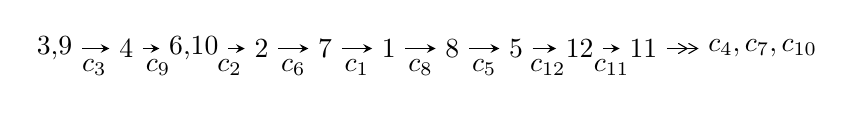
\begin{tikzpicture}[x=23pt, y=7pt]
	% node
	\node (A0) at (-1/8, 0) {3,9};
	\node (A1) at (1, 0) {4};
	\node (A2) at (33/16, 0) {6,10};
	\node (A3) at (25/8, 0) {2};
	\node (A4) at (33/8, 0) {7};
	\node (A5) at (41/8, 0) {1};
	\node (A6) at (49/8, 0) {8};
	\node (A7) at (57/8, 0) {5};
	\node (A8) at (65/8, 0) {12};
	\node (A9) at (73/8, 0) {11};
	\node (C1) at (1/2, -1) {$c_{3}$};
	\node (C2) at (3/2, -1) {$c_{9}$};
	\node (C3) at (21/8, -1) {$c_{2}$};
	\node (C4) at (29/8, -1) {$c_{6}$};
	\node (C5) at (37/8, -1) {$c_{1}$};
	\node (C6) at (45/8, -1) {$c_{8}$};
	\node (C7) at (53/8, -1) {$c_{5}$};
	\node (C8) at (61/8, -1) {$c_{12}$};
	\node (C9) at (69/8, -1) {$c_{11}$};
	\node (A10) at (11, 0) {$c_{4},c_{7},c_{10}$};

	% edge
	\draw[->,>=stealth]	
	(A0) edge (A1) (A1) edge (A2) (A2) edge (A3) (A3) edge (A4) (A4) edge (A5) (A5) edge (A6) (A6) edge (A7) (A7) edge (A8) (A8) edge (A9) ;
	\draw[->>,>={angle 60}]	
	(A9) edge (A10);
\end{tikzpicture} \\ 

\end{tabular} \\

\footnotetext{
The image of knot diagram is generated by the software ``\textbf{Draw programme}" developed by Andrew Bartholomew(\url{http://www.layer8.co.uk/maths/draw/index.htm\#Running-draw}), where we modified some parts for our purpose(\url{https://github.com/CATsTAILs/LinksPainter}).
}\phantom \\ \newline 
\centering \textbf{Ideals for irreducible components\footnotemark of $X_{\text{par}}$} 
 
\begin{align*}
I^u_{1}&=\langle 
-2.58870\times10^{914} u^{158}-4.92785\times10^{914} u^{157}+\cdots+4.36446\times10^{913} b+1.82161\times10^{918},\\
\phantom{I^u_{1}}&\phantom{= \langle  }2.79231\times10^{918} u^{158}+5.30945\times10^{918} u^{157}+\cdots+3.35758\times10^{917} a-1.96428\times10^{922},\\
\phantom{I^u_{1}}&\phantom{= \langle  }u^{159}+3 u^{158}+\cdots-5585 u-7693\rangle \\
I^u_{2}&=\langle 
7.78906\times10^{28} u^{33}+9.44633\times10^{29} u^{32}+\cdots+1.85295\times10^{30} b-1.18903\times10^{30},\\
\phantom{I^u_{2}}&\phantom{= \langle  }1.56226\times10^{30} u^{33}-2.83996\times10^{30} u^{32}+\cdots+1.85295\times10^{30} a-5.33132\times10^{30},\;u^{34}-2 u^{33}+\cdots-2 u+1\rangle \\
\\
\end{align*}
\raggedright * 2 irreducible components of $\dim_{\mathbb{C}}=0$, with total 193 representations.\\
\footnotetext{All coefficients of polynomials are rational numbers. But the coefficients are sometimes approximated in decimal forms when there is not enough margin.}
\newpage
\renewcommand{\arraystretch}{1}
\centering \section*{I. $I^u_{1}= \langle -2.59\times10^{914} u^{158}-4.93\times10^{914} u^{157}+\cdots+4.36\times10^{913} b+1.82\times10^{918},\;2.79\times10^{918} u^{158}+5.31\times10^{918} u^{157}+\cdots+3.36\times10^{917} a-1.96\times10^{922},\;u^{159}+3 u^{158}+\cdots-5585 u-7693 \rangle$}
\flushleft \textbf{(i) Arc colorings}\\
\begin{tabular}{m{7pt} m{180pt} m{7pt} m{180pt} }
\flushright $a_{3}=$&$\begin{pmatrix}1\\0\end{pmatrix}$ \\
\flushright $a_{9}=$&$\begin{pmatrix}0\\u\end{pmatrix}$ \\
\flushright $a_{4}=$&$\begin{pmatrix}1\\- u^2\end{pmatrix}$ \\
\flushright $a_{6}=$&$\begin{pmatrix}-8.31643 u^{158}-15.8133 u^{157}+\cdots-10997.8 u+58502.9\\5.93131 u^{158}+11.2908 u^{157}+\cdots+7878.72 u-41737.3\end{pmatrix}$ \\
\flushright $a_{10}=$&$\begin{pmatrix}u\\- u^3+u\end{pmatrix}$ \\
\flushright $a_{2}=$&$\begin{pmatrix}-8.25706 u^{158}-15.9801 u^{157}+\cdots-12458.3 u+59347.6\\6.00813 u^{158}+11.5632 u^{157}+\cdots+8821.49 u-42858.5\end{pmatrix}$ \\
\flushright $a_{7}=$&$\begin{pmatrix}-19.1831 u^{158}-36.6088 u^{157}+\cdots-25689.8 u+135390.\\10.2278 u^{158}+19.5660 u^{157}+\cdots+14318.7 u-72582.6\end{pmatrix}$ \\
\flushright $a_{1}=$&$\begin{pmatrix}-2.24894 u^{158}-4.41684 u^{157}+\cdots-3636.81 u+16489.2\\6.00813 u^{158}+11.5632 u^{157}+\cdots+8821.49 u-42858.5\end{pmatrix}$ \\
\flushright $a_{8}=$&$\begin{pmatrix}-3.49125 u^{158}-6.39222 u^{157}+\cdots-2490.36 u+23103.1\\-0.614725 u^{158}-1.24739 u^{157}+\cdots-1138.27 u+4569.40\end{pmatrix}$ \\
\flushright $a_{5}=$&$\begin{pmatrix}-1.11875 u^{158}-1.93583 u^{157}+\cdots+640.468 u+6227.96\\-0.643637 u^{158}-1.26257 u^{157}+\cdots-951.234 u+4807.22\end{pmatrix}$ \\
\flushright $a_{12}=$&$\begin{pmatrix}-9.07740 u^{158}-17.5307 u^{157}+\cdots-13309.7 u+64999.7\\7.16040 u^{158}+13.7852 u^{157}+\cdots+10509.8 u-51057.3\end{pmatrix}$ \\
\flushright $a_{11}=$&$\begin{pmatrix}-6.09124 u^{158}-11.8316 u^{157}+\cdots-8380.13 u+43680.5\\3.94321 u^{158}+7.58759 u^{157}+\cdots+5858.27 u-28047.9\end{pmatrix}$\\&\end{tabular}
\flushleft \textbf{(ii) Obstruction class $= -1$}\\~\\
\flushleft \textbf{(iii) Cusp Shapes $= -19.9314 u^{158}-38.0090 u^{157}+\cdots-25810.6 u+139691.$}\\~\\
\newpage\renewcommand{\arraystretch}{1}
\flushleft \textbf{(iv) u-Polynomials at the component}\newline \\
\begin{tabular}{m{50pt}|m{274pt}}
Crossings & \hspace{64pt}u-Polynomials at each crossing \\
\hline $$\begin{aligned}c_{1}\end{aligned}$$&$\begin{aligned}
&u^{159}+64 u^{158}+\cdots-24822244 u-1203409
\end{aligned}$\\
\hline $$\begin{aligned}c_{2},c_{6}\end{aligned}$$&$\begin{aligned}
&u^{159}+32 u^{157}+\cdots+7818 u-1097
\end{aligned}$\\
\hline $$\begin{aligned}c_{3},c_{9}\end{aligned}$$&$\begin{aligned}
&u^{159}+3 u^{158}+\cdots-5585 u-7693
\end{aligned}$\\
\hline $$\begin{aligned}c_{4}\end{aligned}$$&$\begin{aligned}
&u^{159}+5 u^{158}+\cdots-284121 u-279029
\end{aligned}$\\
\hline $$\begin{aligned}c_{5}\end{aligned}$$&$\begin{aligned}
&u^{159}-3 u^{158}+\cdots+3862280 u-51256
\end{aligned}$\\
\hline $$\begin{aligned}c_{7},c_{11}\end{aligned}$$&$\begin{aligned}
&u^{159}- u^{158}+\cdots-4279 u-337
\end{aligned}$\\
\hline $$\begin{aligned}c_{8}\end{aligned}$$&$\begin{aligned}
&u^{159}-3 u^{158}+\cdots+1114751 u-152107
\end{aligned}$\\
\hline $$\begin{aligned}c_{10}\end{aligned}$$&$\begin{aligned}
&u^{159}+u^{158}+\cdots-326007 u-55291
\end{aligned}$\\
\hline $$\begin{aligned}c_{12}\end{aligned}$$&$\begin{aligned}
&u^{159}+17 u^{158}+\cdots+17 u+1
\end{aligned}$\\
\hline
\end{tabular}\\~\\
\newpage\renewcommand{\arraystretch}{1}
\flushleft \textbf{(v) Riley Polynomials at the component}\newline \\
\begin{tabular}{m{50pt}|m{274pt}}
Crossings & \hspace{64pt}Riley Polynomials at each crossing \\
\hline $$\begin{aligned}c_{1}\end{aligned}$$&$\begin{aligned}
&y^{159}+68 y^{158}+\cdots+132998993025548 y-1448193221281
\end{aligned}$\\
\hline $$\begin{aligned}c_{2},c_{6}\end{aligned}$$&$\begin{aligned}
&y^{159}+64 y^{158}+\cdots-24822244 y-1203409
\end{aligned}$\\
\hline $$\begin{aligned}c_{3},c_{9}\end{aligned}$$&$\begin{aligned}
&y^{159}-115 y^{158}+\cdots+852604607 y-59182249
\end{aligned}$\\
\hline $$\begin{aligned}c_{4}\end{aligned}$$&$\begin{aligned}
&y^{159}+27 y^{158}+\cdots-3685160020727 y-77857182841
\end{aligned}$\\
\hline $$\begin{aligned}c_{5}\end{aligned}$$&$\begin{aligned}
&y^{159}-23 y^{158}+\cdots+200629593728 y-2627177536
\end{aligned}$\\
\hline $$\begin{aligned}c_{7},c_{11}\end{aligned}$$&$\begin{aligned}
&y^{159}+87 y^{158}+\cdots+6123921 y-113569
\end{aligned}$\\
\hline $$\begin{aligned}c_{8}\end{aligned}$$&$\begin{aligned}
&y^{159}-55 y^{158}+\cdots+877102825123 y-23136539449
\end{aligned}$\\
\hline $$\begin{aligned}c_{10}\end{aligned}$$&$\begin{aligned}
&y^{159}-35 y^{158}+\cdots-245150469517 y-3057094681
\end{aligned}$\\
\hline $$\begin{aligned}c_{12}\end{aligned}$$&$\begin{aligned}
&y^{159}-21 y^{158}+\cdots-11 y-1
\end{aligned}$\\
\hline
\end{tabular}\\~\\
\newpage\flushleft \textbf{(vi) Complex Volumes and Cusp Shapes}
$$\begin{array}{c|c|c}  
\text{Solutions to }I^u_{1}& \I (\text{vol} + \sqrt{-1}CS) & \text{Cusp shape}\\
 \hline 
\begin{aligned}
u &= -0.998230 + 0.056604 I \\
a &= -0.305260 - 0.965415 I \\
b &= \phantom{-}0.12662 + 1.68847 I\end{aligned}
 & -4.32266 - 0.19712 I & \phantom{-0.000000 } 0 \\ \hline\begin{aligned}
u &= -0.998230 - 0.056604 I \\
a &= -0.305260 + 0.965415 I \\
b &= \phantom{-}0.12662 - 1.68847 I\end{aligned}
 & -4.32266 + 0.19712 I & \phantom{-0.000000 } 0 \\ \hline\begin{aligned}
u &= \phantom{-}0.755548 + 0.696782 I \\
a &= \phantom{-}0.875163 + 0.305869 I \\
b &= -0.303629 - 1.264010 I\end{aligned}
 & -2.06960 + 2.68354 I & \phantom{-0.000000 } 0 \\ \hline\begin{aligned}
u &= \phantom{-}0.755548 - 0.696782 I \\
a &= \phantom{-}0.875163 - 0.305869 I \\
b &= -0.303629 + 1.264010 I\end{aligned}
 & -2.06960 - 2.68354 I & \phantom{-0.000000 } 0 \\ \hline\begin{aligned}
u &= \phantom{-}0.594627 + 0.762529 I \\
a &= \phantom{-}0.039425 + 0.356201 I \\
b &= -0.634948 + 0.986166 I\end{aligned}
 & -3.22180 - 5.85086 I & \phantom{-0.000000 } 0 \\ \hline\begin{aligned}
u &= \phantom{-}0.594627 - 0.762529 I \\
a &= \phantom{-}0.039425 - 0.356201 I \\
b &= -0.634948 - 0.986166 I\end{aligned}
 & -3.22180 + 5.85086 I & \phantom{-0.000000 } 0 \\ \hline\begin{aligned}
u &= -0.210807 + 1.034010 I \\
a &= -0.546647 - 0.382654 I \\
b &= \phantom{-}0.026452 - 1.210650 I\end{aligned}
 & -7.96372 + 6.45459 I & \phantom{-0.000000 } 0 \\ \hline\begin{aligned}
u &= -0.210807 - 1.034010 I \\
a &= -0.546647 + 0.382654 I \\
b &= \phantom{-}0.026452 + 1.210650 I\end{aligned}
 & -7.96372 - 6.45459 I & \phantom{-0.000000 } 0 \\ \hline\begin{aligned}
u &= \phantom{-}0.331910 + 0.876335 I \\
a &= -0.560436 + 0.166825 I \\
b &= \phantom{-}0.685940 - 0.528350 I\end{aligned}
 & \phantom{-}0.69405 + 3.27940 I & \phantom{-0.000000 } 0 \\ \hline\begin{aligned}
u &= \phantom{-}0.331910 - 0.876335 I \\
a &= -0.560436 - 0.166825 I \\
b &= \phantom{-}0.685940 + 0.528350 I\end{aligned}
 & \phantom{-}0.69405 - 3.27940 I & \phantom{-0.000000 } 0\\
 \hline 
 \end{array}$$\newpage$$\begin{array}{c|c|c}  
\text{Solutions to }I^u_{1}& \I (\text{vol} + \sqrt{-1}CS) & \text{Cusp shape}\\
 \hline 
\begin{aligned}
u &= -0.927144 + 0.530437 I \\
a &= \phantom{-}1.44593 - 0.37956 I \\
b &= -0.64661 + 1.26742 I\end{aligned}
 & -3.01406 - 2.12101 I & \phantom{-0.000000 } 0 \\ \hline\begin{aligned}
u &= -0.927144 - 0.530437 I \\
a &= \phantom{-}1.44593 + 0.37956 I \\
b &= -0.64661 - 1.26742 I\end{aligned}
 & -3.01406 + 2.12101 I & \phantom{-0.000000 } 0 \\ \hline\begin{aligned}
u &= \phantom{-}1.07110\phantom{ +0.000000I} \\
a &= \phantom{-}0.943144\phantom{ +0.000000I} \\
b &= -0.495655\phantom{ +0.000000I}\end{aligned}
 & \phantom{-}1.59479\phantom{ +0.000000I} & \phantom{-0.000000 } 0 \\ \hline\begin{aligned}
u &= \phantom{-}1.034070 + 0.301640 I \\
a &= -0.546057 - 0.645865 I \\
b &= \phantom{-}0.034883 - 0.926985 I\end{aligned}
 & \phantom{-}1.95234 + 2.25098 I & \phantom{-0.000000 } 0 \\ \hline\begin{aligned}
u &= \phantom{-}1.034070 - 0.301640 I \\
a &= -0.546057 + 0.645865 I \\
b &= \phantom{-}0.034883 + 0.926985 I\end{aligned}
 & \phantom{-}1.95234 - 2.25098 I & \phantom{-0.000000 } 0 \\ \hline\begin{aligned}
u &= -0.260741 + 1.047610 I \\
a &= -1.072750 - 0.613680 I \\
b &= \phantom{-}0.620672 - 1.030020 I\end{aligned}
 & -0.74335 - 8.33939 I & \phantom{-0.000000 } 0 \\ \hline\begin{aligned}
u &= -0.260741 - 1.047610 I \\
a &= -1.072750 + 0.613680 I \\
b &= \phantom{-}0.620672 + 1.030020 I\end{aligned}
 & -0.74335 + 8.33939 I & \phantom{-0.000000 } 0 \\ \hline\begin{aligned}
u &= -1.029520 + 0.327415 I \\
a &= -0.189237 - 1.014620 I \\
b &= \phantom{-}0.762322 + 0.552008 I\end{aligned}
 & -0.47895 - 4.92362 I & \phantom{-0.000000 } 0 \\ \hline\begin{aligned}
u &= -1.029520 - 0.327415 I \\
a &= -0.189237 + 1.014620 I \\
b &= \phantom{-}0.762322 - 0.552008 I\end{aligned}
 & -0.47895 + 4.92362 I & \phantom{-0.000000 } 0 \\ \hline\begin{aligned}
u &= -0.989286 + 0.434947 I \\
a &= -0.34060 + 1.60831 I \\
b &= -0.146775 + 0.702020 I\end{aligned}
 & -0.40731 - 7.03209 I & \phantom{-0.000000 } 0\\
 \hline 
 \end{array}$$\newpage$$\begin{array}{c|c|c}  
\text{Solutions to }I^u_{1}& \I (\text{vol} + \sqrt{-1}CS) & \text{Cusp shape}\\
 \hline 
\begin{aligned}
u &= -0.989286 - 0.434947 I \\
a &= -0.34060 - 1.60831 I \\
b &= -0.146775 - 0.702020 I\end{aligned}
 & -0.40731 + 7.03209 I & \phantom{-0.000000 } 0 \\ \hline\begin{aligned}
u &= \phantom{-}1.007980 + 0.391765 I \\
a &= -2.14801 + 0.97630 I \\
b &= \phantom{-}0.658038 + 1.048600 I\end{aligned}
 & -1.93511 + 10.31950 I & \phantom{-0.000000 } 0 \\ \hline\begin{aligned}
u &= \phantom{-}1.007980 - 0.391765 I \\
a &= -2.14801 - 0.97630 I \\
b &= \phantom{-}0.658038 - 1.048600 I\end{aligned}
 & -1.93511 - 10.31950 I & \phantom{-0.000000 } 0 \\ \hline\begin{aligned}
u &= -1.084210 + 0.005524 I \\
a &= -2.25931 + 0.90723 I \\
b &= \phantom{-}0.914933 - 0.929006 I\end{aligned}
 & \phantom{-}0.72668 - 2.58040 I & \phantom{-0.000000 } 0 \\ \hline\begin{aligned}
u &= -1.084210 - 0.005524 I \\
a &= -2.25931 - 0.90723 I \\
b &= \phantom{-}0.914933 + 0.929006 I\end{aligned}
 & \phantom{-}0.72668 + 2.58040 I & \phantom{-0.000000 } 0 \\ \hline\begin{aligned}
u &= -1.068790 + 0.214090 I \\
a &= \phantom{-}0.0044551 + 0.0808453 I \\
b &= -0.182360 - 1.328580 I\end{aligned}
 & -5.29763 - 0.05849 I & \phantom{-0.000000 } 0 \\ \hline\begin{aligned}
u &= -1.068790 - 0.214090 I \\
a &= \phantom{-}0.0044551 - 0.0808453 I \\
b &= -0.182360 + 1.328580 I\end{aligned}
 & -5.29763 + 0.05849 I & \phantom{-0.000000 } 0 \\ \hline\begin{aligned}
u &= -0.226550 + 1.068610 I \\
a &= -0.818317 + 0.037390 I \\
b &= \phantom{-}0.819079 + 0.477351 I\end{aligned}
 & -2.06232 - 8.57163 I & \phantom{-0.000000 } 0 \\ \hline\begin{aligned}
u &= -0.226550 - 1.068610 I \\
a &= -0.818317 - 0.037390 I \\
b &= \phantom{-}0.819079 - 0.477351 I\end{aligned}
 & -2.06232 + 8.57163 I & \phantom{-0.000000 } 0 \\ \hline\begin{aligned}
u &= \phantom{-}0.846723 + 0.301804 I \\
a &= \phantom{-}0.765013 - 0.917829 I \\
b &= \phantom{-}0.004476 - 1.127320 I\end{aligned}
 & -6.11695 + 3.56799 I & \phantom{-0.000000 } 0\\
 \hline 
 \end{array}$$\newpage$$\begin{array}{c|c|c}  
\text{Solutions to }I^u_{1}& \I (\text{vol} + \sqrt{-1}CS) & \text{Cusp shape}\\
 \hline 
\begin{aligned}
u &= \phantom{-}0.846723 - 0.301804 I \\
a &= \phantom{-}0.765013 + 0.917829 I \\
b &= \phantom{-}0.004476 + 1.127320 I\end{aligned}
 & -6.11695 - 3.56799 I & \phantom{-0.000000 } 0 \\ \hline\begin{aligned}
u &= -1.028450 + 0.403819 I \\
a &= \phantom{-}0.986638 + 0.435321 I \\
b &= -0.225840 + 0.967325 I\end{aligned}
 & -1.13088 - 2.45330 I & \phantom{-0.000000 } 0 \\ \hline\begin{aligned}
u &= -1.028450 - 0.403819 I \\
a &= \phantom{-}0.986638 - 0.435321 I \\
b &= -0.225840 - 0.967325 I\end{aligned}
 & -1.13088 + 2.45330 I & \phantom{-0.000000 } 0 \\ \hline\begin{aligned}
u &= \phantom{-}0.770144 + 0.439668 I \\
a &= \phantom{-}2.15042 - 0.12942 I \\
b &= -0.127552 - 0.974758 I\end{aligned}
 & -6.40260 - 0.41866 I & \phantom{-0.000000 } 0 \\ \hline\begin{aligned}
u &= \phantom{-}0.770144 - 0.439668 I \\
a &= \phantom{-}2.15042 + 0.12942 I \\
b &= -0.127552 + 0.974758 I\end{aligned}
 & -6.40260 + 0.41866 I & \phantom{-0.000000 } 0 \\ \hline\begin{aligned}
u &= -0.107615 + 0.875901 I \\
a &= -0.243278 + 0.940188 I \\
b &= \phantom{-}0.480889 + 1.034830 I\end{aligned}
 & -6.21376 + 3.91050 I & \phantom{-0.000000 } 0 \\ \hline\begin{aligned}
u &= -0.107615 - 0.875901 I \\
a &= -0.243278 - 0.940188 I \\
b &= \phantom{-}0.480889 - 1.034830 I\end{aligned}
 & -6.21376 - 3.91050 I & \phantom{-0.000000 } 0 \\ \hline\begin{aligned}
u &= -1.119340 + 0.010498 I \\
a &= \phantom{-}3.31565 - 0.12505 I \\
b &= -0.609534 - 0.817153 I\end{aligned}
 & \phantom{-}1.56961 - 4.22958 I & \phantom{-0.000000 } 0 \\ \hline\begin{aligned}
u &= -1.119340 - 0.010498 I \\
a &= \phantom{-}3.31565 + 0.12505 I \\
b &= -0.609534 + 0.817153 I\end{aligned}
 & \phantom{-}1.56961 + 4.22958 I & \phantom{-0.000000 } 0 \\ \hline\begin{aligned}
u &= -0.463833 + 0.744719 I \\
a &= \phantom{-}0.553671 + 0.798452 I \\
b &= -0.663530 + 0.663223 I\end{aligned}
 & -2.24861 + 0.78017 I & \phantom{-0.000000 } 0\\
 \hline 
 \end{array}$$\newpage$$\begin{array}{c|c|c}  
\text{Solutions to }I^u_{1}& \I (\text{vol} + \sqrt{-1}CS) & \text{Cusp shape}\\
 \hline 
\begin{aligned}
u &= -0.463833 - 0.744719 I \\
a &= \phantom{-}0.553671 - 0.798452 I \\
b &= -0.663530 - 0.663223 I\end{aligned}
 & -2.24861 - 0.78017 I & \phantom{-0.000000 } 0 \\ \hline\begin{aligned}
u &= \phantom{-}1.121500 + 0.240629 I \\
a &= -1.72268 - 0.17644 I \\
b &= \phantom{-}1.301470 + 0.287043 I\end{aligned}
 & \phantom{-}1.31700 + 7.23660 I & \phantom{-0.000000 } 0 \\ \hline\begin{aligned}
u &= \phantom{-}1.121500 - 0.240629 I \\
a &= -1.72268 + 0.17644 I \\
b &= \phantom{-}1.301470 - 0.287043 I\end{aligned}
 & \phantom{-}1.31700 - 7.23660 I & \phantom{-0.000000 } 0 \\ \hline\begin{aligned}
u &= \phantom{-}1.145460 + 0.096382 I \\
a &= -2.08745 - 0.91525 I \\
b &= \phantom{-}0.876025 + 1.046550 I\end{aligned}
 & \phantom{-}0.37825 + 4.24541 I & \phantom{-0.000000 } 0 \\ \hline\begin{aligned}
u &= \phantom{-}1.145460 - 0.096382 I \\
a &= -2.08745 + 0.91525 I \\
b &= \phantom{-}0.876025 - 1.046550 I\end{aligned}
 & \phantom{-}0.37825 - 4.24541 I & \phantom{-0.000000 } 0 \\ \hline\begin{aligned}
u &= \phantom{-}1.170950 + 0.120289 I \\
a &= \phantom{-}2.56337 - 0.84885 I \\
b &= -0.580563 - 0.945554 I\end{aligned}
 & \phantom{-}5.02421 + 3.04131 I & \phantom{-0.000000 } 0 \\ \hline\begin{aligned}
u &= \phantom{-}1.170950 - 0.120289 I \\
a &= \phantom{-}2.56337 + 0.84885 I \\
b &= -0.580563 + 0.945554 I\end{aligned}
 & \phantom{-}5.02421 - 3.04131 I & \phantom{-0.000000 } 0 \\ \hline\begin{aligned}
u &= -0.800888 + 0.093377 I \\
a &= \phantom{-}0.879486 + 0.160390 I \\
b &= -0.789295 - 0.645792 I\end{aligned}
 & -0.26494 + 2.40988 I & \phantom{-0.000000 } 0 \\ \hline\begin{aligned}
u &= -0.800888 - 0.093377 I \\
a &= \phantom{-}0.879486 - 0.160390 I \\
b &= -0.789295 + 0.645792 I\end{aligned}
 & -0.26494 - 2.40988 I & \phantom{-0.000000 } 0 \\ \hline\begin{aligned}
u &= -0.101398 + 1.195570 I \\
a &= \phantom{-}0.755610 - 0.083206 I \\
b &= -0.657040 - 0.877020 I\end{aligned}
 & \phantom{-}0.31857 + 1.63483 I & \phantom{-0.000000 } 0\\
 \hline 
 \end{array}$$\newpage$$\begin{array}{c|c|c}  
\text{Solutions to }I^u_{1}& \I (\text{vol} + \sqrt{-1}CS) & \text{Cusp shape}\\
 \hline 
\begin{aligned}
u &= -0.101398 - 1.195570 I \\
a &= \phantom{-}0.755610 + 0.083206 I \\
b &= -0.657040 + 0.877020 I\end{aligned}
 & \phantom{-}0.31857 - 1.63483 I & \phantom{-0.000000 } 0 \\ \hline\begin{aligned}
u &= -1.163570 + 0.319002 I \\
a &= \phantom{-}1.206670 - 0.445892 I \\
b &= -0.238517 - 0.522046 I\end{aligned}
 & -0.14787 + 3.09757 I & \phantom{-0.000000 } 0 \\ \hline\begin{aligned}
u &= -1.163570 - 0.319002 I \\
a &= \phantom{-}1.206670 + 0.445892 I \\
b &= -0.238517 + 0.522046 I\end{aligned}
 & -0.14787 - 3.09757 I & \phantom{-0.000000 } 0 \\ \hline\begin{aligned}
u &= -0.019567 + 0.792817 I \\
a &= -0.397181 + 1.272620 I \\
b &= \phantom{-}0.058253 + 1.040860 I\end{aligned}
 & -4.19818 - 2.06289 I & \phantom{-0.000000 } 0 \\ \hline\begin{aligned}
u &= -0.019567 - 0.792817 I \\
a &= -0.397181 - 1.272620 I \\
b &= \phantom{-}0.058253 - 1.040860 I\end{aligned}
 & -4.19818 + 2.06289 I & \phantom{-0.000000 } 0 \\ \hline\begin{aligned}
u &= \phantom{-}1.209160 + 0.106868 I \\
a &= \phantom{-}1.57776 - 0.14188 I \\
b &= -0.627327 - 1.163320 I\end{aligned}
 & \phantom{-}4.87807 + 4.15319 I & \phantom{-0.000000 } 0 \\ \hline\begin{aligned}
u &= \phantom{-}1.209160 - 0.106868 I \\
a &= \phantom{-}1.57776 + 0.14188 I \\
b &= -0.627327 + 1.163320 I\end{aligned}
 & \phantom{-}4.87807 - 4.15319 I & \phantom{-0.000000 } 0 \\ \hline\begin{aligned}
u &= \phantom{-}0.055245 + 0.777935 I \\
a &= \phantom{-}1.122840 - 0.737605 I \\
b &= -0.655588 - 0.932531 I\end{aligned}
 & -0.08140 + 3.07582 I & \phantom{-0.000000 } 0 \\ \hline\begin{aligned}
u &= \phantom{-}0.055245 - 0.777935 I \\
a &= \phantom{-}1.122840 + 0.737605 I \\
b &= -0.655588 + 0.932531 I\end{aligned}
 & -0.08140 - 3.07582 I & \phantom{-0.000000 } 0 \\ \hline\begin{aligned}
u &= \phantom{-}1.240920 + 0.011755 I \\
a &= -1.86456 - 0.33830 I \\
b &= \phantom{-}0.662989 + 0.919664 I\end{aligned}
 & \phantom{-}4.23313 + 0.35055 I & \phantom{-0.000000 } 0\\
 \hline 
 \end{array}$$\newpage$$\begin{array}{c|c|c}  
\text{Solutions to }I^u_{1}& \I (\text{vol} + \sqrt{-1}CS) & \text{Cusp shape}\\
 \hline 
\begin{aligned}
u &= \phantom{-}1.240920 - 0.011755 I \\
a &= -1.86456 + 0.33830 I \\
b &= \phantom{-}0.662989 - 0.919664 I\end{aligned}
 & \phantom{-}4.23313 - 0.35055 I & \phantom{-0.000000 } 0 \\ \hline\begin{aligned}
u &= \phantom{-}1.241290 + 0.049732 I \\
a &= \phantom{-}1.30674 + 2.17756 I \\
b &= -0.602910 - 0.889713 I\end{aligned}
 & \phantom{-}1.33788 + 9.00851 I & \phantom{-0.000000 } 0 \\ \hline\begin{aligned}
u &= \phantom{-}1.241290 - 0.049732 I \\
a &= \phantom{-}1.30674 - 2.17756 I \\
b &= -0.602910 + 0.889713 I\end{aligned}
 & \phantom{-}1.33788 - 9.00851 I & \phantom{-0.000000 } 0 \\ \hline\begin{aligned}
u &= \phantom{-}1.245610 + 0.055066 I \\
a &= \phantom{-}1.35726 - 0.68550 I \\
b &= -1.108180 + 0.495846 I\end{aligned}
 & \phantom{-}4.06139 + 4.47431 I & \phantom{-0.000000 } 0 \\ \hline\begin{aligned}
u &= \phantom{-}1.245610 - 0.055066 I \\
a &= \phantom{-}1.35726 + 0.68550 I \\
b &= -1.108180 - 0.495846 I\end{aligned}
 & \phantom{-}4.06139 - 4.47431 I & \phantom{-0.000000 } 0 \\ \hline\begin{aligned}
u &= -1.253840 + 0.171329 I \\
a &= -2.62849 + 0.37107 I \\
b &= \phantom{-}0.699047 - 0.918884 I\end{aligned}
 & \phantom{-}4.38909 - 5.88148 I & \phantom{-0.000000 } 0 \\ \hline\begin{aligned}
u &= -1.253840 - 0.171329 I \\
a &= -2.62849 - 0.37107 I \\
b &= \phantom{-}0.699047 + 0.918884 I\end{aligned}
 & \phantom{-}4.38909 + 5.88148 I & \phantom{-0.000000 } 0 \\ \hline\begin{aligned}
u &= \phantom{-}1.261490 + 0.131560 I \\
a &= -1.35271 + 1.60138 I \\
b &= \phantom{-}0.724564 - 0.780989 I\end{aligned}
 & \phantom{-}4.80669 + 0.44565 I & \phantom{-0.000000 } 0 \\ \hline\begin{aligned}
u &= \phantom{-}1.261490 - 0.131560 I \\
a &= -1.35271 - 1.60138 I \\
b &= \phantom{-}0.724564 + 0.780989 I\end{aligned}
 & \phantom{-}4.80669 - 0.44565 I & \phantom{-0.000000 } 0 \\ \hline\begin{aligned}
u &= -1.268540 + 0.079334 I \\
a &= \phantom{-}0.18558 + 2.09686 I \\
b &= -0.540326 - 0.776382 I\end{aligned}
 & \phantom{-}5.61646 + 1.44960 I & \phantom{-0.000000 } 0\\
 \hline 
 \end{array}$$\newpage$$\begin{array}{c|c|c}  
\text{Solutions to }I^u_{1}& \I (\text{vol} + \sqrt{-1}CS) & \text{Cusp shape}\\
 \hline 
\begin{aligned}
u &= -1.268540 - 0.079334 I \\
a &= \phantom{-}0.18558 - 2.09686 I \\
b &= -0.540326 + 0.776382 I\end{aligned}
 & \phantom{-}5.61646 - 1.44960 I & \phantom{-0.000000 } 0 \\ \hline\begin{aligned}
u &= -1.259180 + 0.185861 I \\
a &= \phantom{-}1.81294 - 0.21631 I \\
b &= -0.754992 + 1.181590 I\end{aligned}
 & \phantom{-}1.92301 - 11.09530 I & \phantom{-0.000000 } 0 \\ \hline\begin{aligned}
u &= -1.259180 - 0.185861 I \\
a &= \phantom{-}1.81294 + 0.21631 I \\
b &= -0.754992 - 1.181590 I\end{aligned}
 & \phantom{-}1.92301 + 11.09530 I & \phantom{-0.000000 } 0 \\ \hline\begin{aligned}
u &= -0.263817 + 0.668835 I \\
a &= \phantom{-}0.588389 + 0.026754 I \\
b &= -0.608365 - 0.811386 I\end{aligned}
 & \phantom{-}0.36170 + 1.89276 I & \phantom{-0.000000 } 0 \\ \hline\begin{aligned}
u &= -0.263817 - 0.668835 I \\
a &= \phantom{-}0.588389 - 0.026754 I \\
b &= -0.608365 + 0.811386 I\end{aligned}
 & \phantom{-}0.36170 - 1.89276 I & \phantom{-0.000000 } 0 \\ \hline\begin{aligned}
u &= -1.283580 + 0.012359 I \\
a &= \phantom{-}0.839158 - 0.724273 I \\
b &= -0.808124 + 0.465228 I\end{aligned}
 & \phantom{-}7.02134 - 1.27085 I & \phantom{-0.000000 } 0 \\ \hline\begin{aligned}
u &= -1.283580 - 0.012359 I \\
a &= \phantom{-}0.839158 + 0.724273 I \\
b &= -0.808124 - 0.465228 I\end{aligned}
 & \phantom{-}7.02134 + 1.27085 I & \phantom{-0.000000 } 0 \\ \hline\begin{aligned}
u &= \phantom{-}1.280260 + 0.114855 I \\
a &= -1.45072 + 0.78969 I \\
b &= \phantom{-}0.800436 - 0.852565 I\end{aligned}
 & \phantom{-}4.51874 - 0.16581 I & \phantom{-0.000000 } 0 \\ \hline\begin{aligned}
u &= \phantom{-}1.280260 - 0.114855 I \\
a &= -1.45072 - 0.78969 I \\
b &= \phantom{-}0.800436 + 0.852565 I\end{aligned}
 & \phantom{-}4.51874 + 0.16581 I & \phantom{-0.000000 } 0 \\ \hline\begin{aligned}
u &= \phantom{-}0.205143 + 1.270010 I \\
a &= -0.953570 + 0.304264 I \\
b &= \phantom{-}0.650565 + 1.088450 I\end{aligned}
 & -3.8636 + 14.0598 I & \phantom{-0.000000 } 0\\
 \hline 
 \end{array}$$\newpage$$\begin{array}{c|c|c}  
\text{Solutions to }I^u_{1}& \I (\text{vol} + \sqrt{-1}CS) & \text{Cusp shape}\\
 \hline 
\begin{aligned}
u &= \phantom{-}0.205143 - 1.270010 I \\
a &= -0.953570 - 0.304264 I \\
b &= \phantom{-}0.650565 - 1.088450 I\end{aligned}
 & -3.8636 - 14.0598 I & \phantom{-0.000000 } 0 \\ \hline\begin{aligned}
u &= \phantom{-}1.249030 + 0.313432 I \\
a &= \phantom{-}0.800746 - 0.476986 I \\
b &= -0.824676 + 0.214340 I\end{aligned}
 & -0.14374 + 3.65613 I & \phantom{-0.000000 } 0 \\ \hline\begin{aligned}
u &= \phantom{-}1.249030 - 0.313432 I \\
a &= \phantom{-}0.800746 + 0.476986 I \\
b &= -0.824676 - 0.214340 I\end{aligned}
 & -0.14374 - 3.65613 I & \phantom{-0.000000 } 0 \\ \hline\begin{aligned}
u &= \phantom{-}1.236870 + 0.372862 I \\
a &= -0.493892 + 0.126708 I \\
b &= \phantom{-}0.041339 + 1.196340 I\end{aligned}
 & -0.39157 + 6.26546 I & \phantom{-0.000000 } 0 \\ \hline\begin{aligned}
u &= \phantom{-}1.236870 - 0.372862 I \\
a &= -0.493892 - 0.126708 I \\
b &= \phantom{-}0.041339 - 1.196340 I\end{aligned}
 & -0.39157 - 6.26546 I & \phantom{-0.000000 } 0 \\ \hline\begin{aligned}
u &= -1.278050 + 0.229073 I \\
a &= -2.00152 + 0.44928 I \\
b &= \phantom{-}0.739935 - 0.905459 I\end{aligned}
 & \phantom{-}4.32573 - 5.61032 I & \phantom{-0.000000 } 0 \\ \hline\begin{aligned}
u &= -1.278050 - 0.229073 I \\
a &= -2.00152 - 0.44928 I \\
b &= \phantom{-}0.739935 + 0.905459 I\end{aligned}
 & \phantom{-}4.32573 + 5.61032 I & \phantom{-0.000000 } 0 \\ \hline\begin{aligned}
u &= -1.198420 + 0.511893 I \\
a &= -0.683459 + 0.146140 I \\
b &= \phantom{-}0.174514 - 1.327100 I\end{aligned}
 & -4.85586 - 11.87490 I & \phantom{-0.000000 } 0 \\ \hline\begin{aligned}
u &= -1.198420 - 0.511893 I \\
a &= -0.683459 - 0.146140 I \\
b &= \phantom{-}0.174514 + 1.327100 I\end{aligned}
 & -4.85586 + 11.87490 I & \phantom{-0.000000 } 0 \\ \hline\begin{aligned}
u &= -1.238580 + 0.417998 I \\
a &= \phantom{-}1.73426 + 0.47324 I \\
b &= -0.561304 + 1.106100 I\end{aligned}
 & -2.68541 - 8.54615 I & \phantom{-0.000000 } 0\\
 \hline 
 \end{array}$$\newpage$$\begin{array}{c|c|c}  
\text{Solutions to }I^u_{1}& \I (\text{vol} + \sqrt{-1}CS) & \text{Cusp shape}\\
 \hline 
\begin{aligned}
u &= -1.238580 - 0.417998 I \\
a &= \phantom{-}1.73426 - 0.47324 I \\
b &= -0.561304 - 1.106100 I\end{aligned}
 & -2.68541 + 8.54615 I & \phantom{-0.000000 } 0 \\ \hline\begin{aligned}
u &= -0.015696 + 0.684873 I \\
a &= \phantom{-}0.043489 + 0.639741 I \\
b &= \phantom{-}0.544402 + 0.177566 I\end{aligned}
 & -4.00879 - 0.00094 I & \phantom{-0.000000 } 0 \\ \hline\begin{aligned}
u &= -0.015696 - 0.684873 I \\
a &= \phantom{-}0.043489 - 0.639741 I \\
b &= \phantom{-}0.544402 - 0.177566 I\end{aligned}
 & -4.00879 + 0.00094 I & \phantom{-0.000000 } 0 \\ \hline\begin{aligned}
u &= \phantom{-}1.285200 + 0.298812 I \\
a &= -0.530389 - 1.181650 I \\
b &= -0.308619 + 0.784211 I\end{aligned}
 & -0.42326 + 5.17727 I & \phantom{-0.000000 } 0 \\ \hline\begin{aligned}
u &= \phantom{-}1.285200 - 0.298812 I \\
a &= -0.530389 + 1.181650 I \\
b &= -0.308619 - 0.784211 I\end{aligned}
 & -0.42326 - 5.17727 I & \phantom{-0.000000 } 0 \\ \hline\begin{aligned}
u &= \phantom{-}0.358641 + 0.573632 I \\
a &= \phantom{-}1.035120 + 0.380710 I \\
b &= -0.368695 + 0.030136 I\end{aligned}
 & \phantom{-}0.872410 + 0.982789 I & \phantom{-0.000000 } 0 \\ \hline\begin{aligned}
u &= \phantom{-}0.358641 - 0.573632 I \\
a &= \phantom{-}1.035120 - 0.380710 I \\
b &= -0.368695 - 0.030136 I\end{aligned}
 & \phantom{-}0.872410 - 0.982789 I & \phantom{-0.000000 } 0 \\ \hline\begin{aligned}
u &= -1.329220 + 0.226197 I \\
a &= -1.084910 + 0.254471 I \\
b &= \phantom{-}0.674735 - 0.248436 I\end{aligned}
 & \phantom{-}4.98883 - 4.27401 I & \phantom{-0.000000 } 0 \\ \hline\begin{aligned}
u &= -1.329220 - 0.226197 I \\
a &= -1.084910 - 0.254471 I \\
b &= \phantom{-}0.674735 + 0.248436 I\end{aligned}
 & \phantom{-}4.98883 + 4.27401 I & \phantom{-0.000000 } 0 \\ \hline\begin{aligned}
u &= -0.375116 + 0.515641 I \\
a &= -2.30431 - 0.56324 I \\
b &= \phantom{-}0.307512 - 1.083760 I\end{aligned}
 & -7.33839 - 2.83916 I & \phantom{-0.000000 } 0\\
 \hline 
 \end{array}$$\newpage$$\begin{array}{c|c|c}  
\text{Solutions to }I^u_{1}& \I (\text{vol} + \sqrt{-1}CS) & \text{Cusp shape}\\
 \hline 
\begin{aligned}
u &= -0.375116 - 0.515641 I \\
a &= -2.30431 + 0.56324 I \\
b &= \phantom{-}0.307512 + 1.083760 I\end{aligned}
 & -7.33839 + 2.83916 I & \phantom{-0.000000 } 0 \\ \hline\begin{aligned}
u &= -0.175734 + 0.581083 I \\
a &= \phantom{-}0.763350 - 0.171263 I \\
b &= \phantom{-}0.268253 + 1.071510 I\end{aligned}
 & -4.73018 - 1.86025 I & \phantom{-0.000000 } 0 \\ \hline\begin{aligned}
u &= -0.175734 - 0.581083 I \\
a &= \phantom{-}0.763350 + 0.171263 I \\
b &= \phantom{-}0.268253 - 1.071510 I\end{aligned}
 & -4.73018 + 1.86025 I & \phantom{-0.000000 } 0 \\ \hline\begin{aligned}
u &= -1.385180 + 0.155061 I \\
a &= \phantom{-}0.802320 + 0.298138 I \\
b &= -0.235301 + 0.611966 I\end{aligned}
 & -0.28888 - 3.13725 I & \phantom{-0.000000 } 0 \\ \hline\begin{aligned}
u &= -1.385180 - 0.155061 I \\
a &= \phantom{-}0.802320 - 0.298138 I \\
b &= -0.235301 - 0.611966 I\end{aligned}
 & -0.28888 + 3.13725 I & \phantom{-0.000000 } 0 \\ \hline\begin{aligned}
u &= -1.42109 + 0.10749 I \\
a &= -1.107990 + 0.769973 I \\
b &= \phantom{-}0.599310 - 0.722376 I\end{aligned}
 & \phantom{-}4.87228 - 4.68602 I & \phantom{-0.000000 } 0 \\ \hline\begin{aligned}
u &= -1.42109 - 0.10749 I \\
a &= -1.107990 - 0.769973 I \\
b &= \phantom{-}0.599310 + 0.722376 I\end{aligned}
 & \phantom{-}4.87228 + 4.68602 I & \phantom{-0.000000 } 0 \\ \hline\begin{aligned}
u &= -1.38287 + 0.42808 I \\
a &= -1.251540 - 0.599889 I \\
b &= \phantom{-}0.980732 + 0.486269 I\end{aligned}
 & \phantom{-}6.16081 - 5.31879 I & \phantom{-0.000000 } 0 \\ \hline\begin{aligned}
u &= -1.38287 - 0.42808 I \\
a &= -1.251540 + 0.599889 I \\
b &= \phantom{-}0.980732 - 0.486269 I\end{aligned}
 & \phantom{-}6.16081 + 5.31879 I & \phantom{-0.000000 } 0 \\ \hline\begin{aligned}
u &= \phantom{-}1.41457 + 0.38947 I \\
a &= -1.14148 + 0.87019 I \\
b &= \phantom{-}0.909295 - 0.681033 I\end{aligned}
 & \phantom{-}6.58811 + 1.81713 I & \phantom{-0.000000 } 0\\
 \hline 
 \end{array}$$\newpage$$\begin{array}{c|c|c}  
\text{Solutions to }I^u_{1}& \I (\text{vol} + \sqrt{-1}CS) & \text{Cusp shape}\\
 \hline 
\begin{aligned}
u &= \phantom{-}1.41457 - 0.38947 I \\
a &= -1.14148 - 0.87019 I \\
b &= \phantom{-}0.909295 + 0.681033 I\end{aligned}
 & \phantom{-}6.58811 - 1.81713 I & \phantom{-0.000000 } 0 \\ \hline\begin{aligned}
u &= -1.41994 + 0.38959 I \\
a &= \phantom{-}0.994183 + 0.913820 I \\
b &= -0.873194 - 0.560161 I\end{aligned}
 & \phantom{-}6.13762 - 7.87850 I & \phantom{-0.000000 } 0 \\ \hline\begin{aligned}
u &= -1.41994 - 0.38959 I \\
a &= \phantom{-}0.994183 - 0.913820 I \\
b &= -0.873194 + 0.560161 I\end{aligned}
 & \phantom{-}6.13762 + 7.87850 I & \phantom{-0.000000 } 0 \\ \hline\begin{aligned}
u &= \phantom{-}1.42157 + 0.47243 I \\
a &= \phantom{-}1.120800 - 0.859041 I \\
b &= -0.988226 + 0.576306 I\end{aligned}
 & \phantom{-}3.0579 + 14.0234 I & \phantom{-0.000000 } 0 \\ \hline\begin{aligned}
u &= \phantom{-}1.42157 - 0.47243 I \\
a &= \phantom{-}1.120800 + 0.859041 I \\
b &= -0.988226 - 0.576306 I\end{aligned}
 & \phantom{-}3.0579 - 14.0234 I & \phantom{-0.000000 } 0 \\ \hline\begin{aligned}
u &= \phantom{-}0.377555 + 0.328668 I \\
a &= \phantom{-}1.86659 - 1.42322 I \\
b &= -0.975459 + 0.687135 I\end{aligned}
 & -0.95796 - 4.69135 I & \phantom{-0.000000 -}0. + 9.65657 I \\ \hline\begin{aligned}
u &= \phantom{-}0.377555 - 0.328668 I \\
a &= \phantom{-}1.86659 + 1.42322 I \\
b &= -0.975459 - 0.687135 I\end{aligned}
 & -0.95796 + 4.69135 I & \phantom{-0.000000 } 0. - 9.65657 I \\ \hline\begin{aligned}
u &= \phantom{-}0.494676 + 0.039149 I \\
a &= \phantom{-}0.608157 - 0.438955 I \\
b &= -0.664879 + 1.095290 I\end{aligned}
 & -1.70446 - 3.38880 I & \phantom{-}4.00000 + 0. I\phantom{ +0.000000I} \\ \hline\begin{aligned}
u &= \phantom{-}0.494676 - 0.039149 I \\
a &= \phantom{-}0.608157 + 0.438955 I \\
b &= -0.664879 - 1.095290 I\end{aligned}
 & -1.70446 + 3.38880 I & \phantom{-}4.00000 + 0. I\phantom{ +0.000000I} \\ \hline\begin{aligned}
u &= \phantom{-}1.43311 + 0.45810 I \\
a &= \phantom{-}1.94979 - 0.10603 I \\
b &= -0.693002 - 1.087090 I\end{aligned}
 & \phantom{-}4.5317 + 13.6898 I & \phantom{-0.000000 } 0\\
 \hline 
 \end{array}$$\newpage$$\begin{array}{c|c|c}  
\text{Solutions to }I^u_{1}& \I (\text{vol} + \sqrt{-1}CS) & \text{Cusp shape}\\
 \hline 
\begin{aligned}
u &= \phantom{-}1.43311 - 0.45810 I \\
a &= \phantom{-}1.94979 + 0.10603 I \\
b &= -0.693002 + 1.087090 I\end{aligned}
 & \phantom{-}4.5317 - 13.6898 I & \phantom{-0.000000 } 0 \\ \hline\begin{aligned}
u &= -1.43238 + 0.47747 I \\
a &= -1.90101 + 0.02286 I \\
b &= \phantom{-}0.750615 - 1.043010 I\end{aligned}
 & \phantom{-}5.45362 - 7.92777 I & \phantom{-0.000000 } 0 \\ \hline\begin{aligned}
u &= -1.43238 - 0.47747 I \\
a &= -1.90101 - 0.02286 I \\
b &= \phantom{-}0.750615 + 1.043010 I\end{aligned}
 & \phantom{-}5.45362 + 7.92777 I & \phantom{-0.000000 } 0 \\ \hline\begin{aligned}
u &= -0.12850 + 1.50976 I \\
a &= \phantom{-}1.000350 - 0.272130 I \\
b &= -0.624161 - 0.809222 I\end{aligned}
 & \phantom{-}0.52767 + 3.38319 I & \phantom{-0.000000 } 0 \\ \hline\begin{aligned}
u &= -0.12850 - 1.50976 I \\
a &= \phantom{-}1.000350 + 0.272130 I \\
b &= -0.624161 + 0.809222 I\end{aligned}
 & \phantom{-}0.52767 - 3.38319 I & \phantom{-0.000000 } 0 \\ \hline\begin{aligned}
u &= \phantom{-}0.060754 + 0.475717 I \\
a &= \phantom{-}0.680605 + 0.814523 I \\
b &= -0.584284 - 0.472779 I\end{aligned}
 & \phantom{-}0.61126 + 1.48879 I & \phantom{-}6.01391 - 4.96004 I \\ \hline\begin{aligned}
u &= \phantom{-}0.060754 - 0.475717 I \\
a &= \phantom{-}0.680605 - 0.814523 I \\
b &= -0.584284 + 0.472779 I\end{aligned}
 & \phantom{-}0.61126 - 1.48879 I & \phantom{-}6.01391 + 4.96004 I \\ \hline\begin{aligned}
u &= \phantom{-}1.42760 + 0.54533 I \\
a &= -0.795754 + 0.827410 I \\
b &= \phantom{-}0.781138 - 0.790563 I\end{aligned}
 & \phantom{-}4.99762 + 4.56492 I & \phantom{-0.000000 } 0 \\ \hline\begin{aligned}
u &= \phantom{-}1.42760 - 0.54533 I \\
a &= -0.795754 - 0.827410 I \\
b &= \phantom{-}0.781138 + 0.790563 I\end{aligned}
 & \phantom{-}4.99762 - 4.56492 I & \phantom{-0.000000 } 0 \\ \hline\begin{aligned}
u &= -1.39875 + 0.63574 I \\
a &= -1.78996 - 0.28475 I \\
b &= \phantom{-}0.731904 - 0.940504 I\end{aligned}
 & \phantom{-}4.53033 - 10.27560 I & \phantom{-0.000000 } 0\\
 \hline 
 \end{array}$$\newpage$$\begin{array}{c|c|c}  
\text{Solutions to }I^u_{1}& \I (\text{vol} + \sqrt{-1}CS) & \text{Cusp shape}\\
 \hline 
\begin{aligned}
u &= -1.39875 - 0.63574 I \\
a &= -1.78996 + 0.28475 I \\
b &= \phantom{-}0.731904 + 0.940504 I\end{aligned}
 & \phantom{-}4.53033 + 10.27560 I & \phantom{-0.000000 } 0 \\ \hline\begin{aligned}
u &= -1.46201 + 0.53500 I \\
a &= \phantom{-}1.88190 - 0.00198 I \\
b &= -0.737831 + 1.125560 I\end{aligned}
 & \phantom{-}1.3350 - 20.3047 I & \phantom{-0.000000 } 0 \\ \hline\begin{aligned}
u &= -1.46201 - 0.53500 I \\
a &= \phantom{-}1.88190 + 0.00198 I \\
b &= -0.737831 - 1.125560 I\end{aligned}
 & \phantom{-}1.3350 + 20.3047 I & \phantom{-0.000000 } 0 \\ \hline\begin{aligned}
u &= \phantom{-}1.45420 + 0.57975 I \\
a &= -1.60649 + 0.33605 I \\
b &= \phantom{-}0.597537 + 0.922893 I\end{aligned}
 & \phantom{-}4.65572 + 6.98413 I & \phantom{-0.000000 } 0 \\ \hline\begin{aligned}
u &= \phantom{-}1.45420 - 0.57975 I \\
a &= -1.60649 - 0.33605 I \\
b &= \phantom{-}0.597537 - 0.922893 I\end{aligned}
 & \phantom{-}4.65572 - 6.98413 I & \phantom{-0.000000 } 0 \\ \hline\begin{aligned}
u &= \phantom{-}1.47628 + 0.56010 I \\
a &= -1.67532 - 0.13368 I \\
b &= \phantom{-}0.707049 + 1.134670 I\end{aligned}
 & \phantom{-}4.18893 + 11.42150 I & \phantom{-0.000000 } 0 \\ \hline\begin{aligned}
u &= \phantom{-}1.47628 - 0.56010 I \\
a &= -1.67532 + 0.13368 I \\
b &= \phantom{-}0.707049 - 1.134670 I\end{aligned}
 & \phantom{-}4.18893 - 11.42150 I & \phantom{-0.000000 } 0 \\ \hline\begin{aligned}
u &= -1.54415 + 0.44438 I \\
a &= -0.667840 - 0.731079 I \\
b &= \phantom{-}0.575105 + 0.778621 I\end{aligned}
 & \phantom{-}5.13375 - 2.31436 I & \phantom{-0.000000 } 0 \\ \hline\begin{aligned}
u &= -1.54415 - 0.44438 I \\
a &= -0.667840 + 0.731079 I \\
b &= \phantom{-}0.575105 - 0.778621 I\end{aligned}
 & \phantom{-}5.13375 + 2.31436 I & \phantom{-0.000000 } 0 \\ \hline\begin{aligned}
u &= -0.375435 + 0.064149 I \\
a &= \phantom{-}5.55414 + 1.85182 I \\
b &= \phantom{-}0.002629 + 0.664397 I\end{aligned}
 & -4.77694 - 1.09489 I & -0.60906 + 8.24374 I\\
 \hline 
 \end{array}$$\newpage$$\begin{array}{c|c|c}  
\text{Solutions to }I^u_{1}& \I (\text{vol} + \sqrt{-1}CS) & \text{Cusp shape}\\
 \hline 
\begin{aligned}
u &= -0.375435 - 0.064149 I \\
a &= \phantom{-}5.55414 - 1.85182 I \\
b &= \phantom{-}0.002629 - 0.664397 I\end{aligned}
 & -4.77694 + 1.09489 I & -0.60906 - 8.24374 I \\ \hline\begin{aligned}
u &= \phantom{-}0.238701 + 0.217595 I \\
a &= \phantom{-}3.00357 - 1.12547 I \\
b &= \phantom{-}0.528584 - 0.724297 I\end{aligned}
 & \phantom{-}2.31513 - 1.60194 I & \phantom{-}7.58569 - 4.88635 I \\ \hline\begin{aligned}
u &= \phantom{-}0.238701 - 0.217595 I \\
a &= \phantom{-}3.00357 + 1.12547 I \\
b &= \phantom{-}0.528584 + 0.724297 I\end{aligned}
 & \phantom{-}2.31513 + 1.60194 I & \phantom{-}7.58569 + 4.88635 I \\ \hline\begin{aligned}
u &= -0.318100 + 0.003896 I \\
a &= \phantom{-}2.05695 + 0.98958 I \\
b &= \phantom{-}0.695973 - 0.454890 I\end{aligned}
 & -0.38959 + 4.08543 I & \phantom{-}4.80991 - 2.78422 I \\ \hline\begin{aligned}
u &= -0.318100 - 0.003896 I \\
a &= \phantom{-}2.05695 - 0.98958 I \\
b &= \phantom{-}0.695973 + 0.454890 I\end{aligned}
 & -0.38959 - 4.08543 I & \phantom{-}4.80991 + 2.78422 I \\ \hline\begin{aligned}
u &= \phantom{-}0.10372 + 1.68534 I \\
a &= \phantom{-}0.710432 + 0.039211 I \\
b &= -0.521295 + 0.999211 I\end{aligned}
 & -0.93111 - 4.39304 I & \phantom{-0.000000 } 0 \\ \hline\begin{aligned}
u &= \phantom{-}0.10372 - 1.68534 I \\
a &= \phantom{-}0.710432 - 0.039211 I \\
b &= -0.521295 - 0.999211 I\end{aligned}
 & -0.93111 + 4.39304 I & \phantom{-0.000000 } 0 \\ \hline\begin{aligned}
u &= \phantom{-}0.072203 + 0.287898 I \\
a &= \phantom{-}3.11145 - 0.49790 I \\
b &= \phantom{-}0.531189 - 0.971492 I\end{aligned}
 & \phantom{-}1.52091 - 2.70354 I & -3.36689 + 10.25142 I \\ \hline\begin{aligned}
u &= \phantom{-}0.072203 - 0.287898 I \\
a &= \phantom{-}3.11145 + 0.49790 I \\
b &= \phantom{-}0.531189 + 0.971492 I\end{aligned}
 & \phantom{-}1.52091 + 2.70354 I & -3.36689 - 10.25142 I \\ \hline\begin{aligned}
u &= \phantom{-}1.71037 + 0.24675 I \\
a &= \phantom{-}0.520132 - 0.273181 I \\
b &= -0.337170 + 0.857973 I\end{aligned}
 & -0.812201 + 0.684522 I & \phantom{-0.000000 } 0\\
 \hline 
 \end{array}$$\newpage$$\begin{array}{c|c|c}  
\text{Solutions to }I^u_{1}& \I (\text{vol} + \sqrt{-1}CS) & \text{Cusp shape}\\
 \hline 
\begin{aligned}
u &= \phantom{-}1.71037 - 0.24675 I \\
a &= \phantom{-}0.520132 + 0.273181 I \\
b &= -0.337170 - 0.857973 I\end{aligned}
 & -0.812201 - 0.684522 I & \phantom{-0.000000 } 0 \\ \hline\begin{aligned}
u &= \phantom{-}0.089842 + 0.243647 I \\
a &= \phantom{-}1.64776 + 2.66269 I \\
b &= \phantom{-}0.614847 + 1.077680 I\end{aligned}
 & -2.17842 + 9.17430 I & \phantom{-}1.82314 - 6.56921 I \\ \hline\begin{aligned}
u &= \phantom{-}0.089842 - 0.243647 I \\
a &= \phantom{-}1.64776 - 2.66269 I \\
b &= \phantom{-}0.614847 - 1.077680 I\end{aligned}
 & -2.17842 - 9.17430 I & \phantom{-}1.82314 + 6.56921 I \\ \hline\begin{aligned}
u &= -1.90614 + 0.21575 I \\
a &= \phantom{-}1.55686 - 0.17208 I \\
b &= -0.570536 + 0.806652 I\end{aligned}
 & \phantom{-}0.903909 + 0.431493 I & \phantom{-0.000000 } 0 \\ \hline\begin{aligned}
u &= -1.90614 - 0.21575 I \\
a &= \phantom{-}1.55686 + 0.17208 I \\
b &= -0.570536 - 0.806652 I\end{aligned}
 & \phantom{-}0.903909 - 0.431493 I & \phantom{-0.000000 } 0 \\ \hline\begin{aligned}
u &= \phantom{-}2.00152 + 0.05404 I \\
a &= \phantom{-}1.281640 - 0.515843 I \\
b &= -0.574496 + 0.902340 I\end{aligned}
 & \phantom{-}0.58953 - 4.99476 I & \phantom{-0.000000 } 0 \\ \hline\begin{aligned}
u &= \phantom{-}2.00152 - 0.05404 I \\
a &= \phantom{-}1.281640 + 0.515843 I \\
b &= -0.574496 - 0.902340 I\end{aligned}
 & \phantom{-}0.58953 + 4.99476 I & \phantom{-0.000000 } 0 \\ \hline\begin{aligned}
u &= \phantom{-}0.25425 + 2.43540 I \\
a &= \phantom{-}0.933225 + 0.284927 I \\
b &= -0.461292 + 0.776100 I\end{aligned}
 & -0.056205 + 0.448439 I & \phantom{-0.000000 } 0 \\ \hline\begin{aligned}
u &= \phantom{-}0.25425 - 2.43540 I \\
a &= \phantom{-}0.933225 - 0.284927 I \\
b &= -0.461292 - 0.776100 I\end{aligned}
 & -0.056205 - 0.448439 I & \phantom{-0.000000 } 0\\
 \hline 
 \end{array}$$\newpage\newpage\renewcommand{\arraystretch}{1}
\centering \section*{II. $I^u_{2}= \langle 7.79\times10^{28} u^{33}+9.45\times10^{29} u^{32}+\cdots+1.85\times10^{30} b-1.19\times10^{30},\;1.56\times10^{30} u^{33}-2.84\times10^{30} u^{32}+\cdots+1.85\times10^{30} a-5.33\times10^{30},\;u^{34}-2 u^{33}+\cdots-2 u+1 \rangle$}
\flushleft \textbf{(i) Arc colorings}\\
\begin{tabular}{m{7pt} m{180pt} m{7pt} m{180pt} }
\flushright $a_{3}=$&$\begin{pmatrix}1\\0\end{pmatrix}$ \\
\flushright $a_{9}=$&$\begin{pmatrix}0\\u\end{pmatrix}$ \\
\flushright $a_{4}=$&$\begin{pmatrix}1\\- u^2\end{pmatrix}$ \\
\flushright $a_{6}=$&$\begin{pmatrix}-0.843122 u^{33}+1.53267 u^{32}+\cdots-3.82545 u+2.87721\\-0.0420360 u^{33}-0.509800 u^{32}+\cdots-4.00410 u+0.641699\end{pmatrix}$ \\
\flushright $a_{10}=$&$\begin{pmatrix}u\\- u^3+u\end{pmatrix}$ \\
\flushright $a_{2}=$&$\begin{pmatrix}0.123433 u^{33}-1.18111 u^{32}+\cdots-6.24049 u+2.01955\\0.774671 u^{33}-0.993673 u^{32}+\cdots+2.48256 u-1.91740\end{pmatrix}$ \\
\flushright $a_{7}=$&$\begin{pmatrix}0.293023 u^{33}-1.37709 u^{32}+\cdots-2.17885 u-0.692909\\-0.168391 u^{33}+1.12477 u^{32}+\cdots+1.18168 u+1.03755\end{pmatrix}$ \\
\flushright $a_{1}=$&$\begin{pmatrix}0.898104 u^{33}-2.17478 u^{32}+\cdots-3.75793 u+0.102148\\0.774671 u^{33}-0.993673 u^{32}+\cdots+2.48256 u-1.91740\end{pmatrix}$ \\
\flushright $a_{8}=$&$\begin{pmatrix}-1.54514 u^{33}+2.72030 u^{32}+\cdots+0.367285 u-0.132372\\-0.122956 u^{33}+0.431436 u^{32}+\cdots+2.05304 u-1.88832\end{pmatrix}$ \\
\flushright $a_{5}=$&$\begin{pmatrix}-0.574428 u^{33}+1.75434 u^{32}+\cdots+7.10548 u-0.260983\\-0.456970 u^{33}+0.655203 u^{32}+\cdots-0.918090 u-0.578563\end{pmatrix}$ \\
\flushright $a_{12}=$&$\begin{pmatrix}0.335647 u^{33}-1.64076 u^{32}+\cdots-5.38566 u+1.02002\\1.04455 u^{33}-1.56367 u^{32}+\cdots+1.47416 u-1.59042\end{pmatrix}$ \\
\flushright $a_{11}=$&$\begin{pmatrix}0.317307 u^{33}-1.83073 u^{32}+\cdots-6.85640 u-0.552115\\1.31326 u^{33}-2.17579 u^{32}+\cdots+4.44259 u-1.62039\end{pmatrix}$\\&\end{tabular}
\flushleft \textbf{(ii) Obstruction class $= 1$}\\~\\
\flushleft \textbf{(iii) Cusp Shapes $= -0.312721 u^{33}-4.02626 u^{32}+\cdots-16.9736 u+4.08663$}\\~\\
\newpage\renewcommand{\arraystretch}{1}
\flushleft \textbf{(iv) u-Polynomials at the component}\newline \\
\begin{tabular}{m{50pt}|m{274pt}}
Crossings & \hspace{64pt}u-Polynomials at each crossing \\
\hline $$\begin{aligned}c_{1}\end{aligned}$$&$\begin{aligned}
&u^{34}-17 u^{33}+\cdots-11 u+1
\end{aligned}$\\
\hline $$\begin{aligned}c_{2}\end{aligned}$$&$\begin{aligned}
&u^{34}-3 u^{33}+\cdots-5 u+1
\end{aligned}$\\
\hline $$\begin{aligned}c_{3}\end{aligned}$$&$\begin{aligned}
&u^{34}-2 u^{33}+\cdots-2 u+1
\end{aligned}$\\
\hline $$\begin{aligned}c_{4}\end{aligned}$$&$\begin{aligned}
&u^{34}+2 u^{32}+\cdots+12 u+1
\end{aligned}$\\
\hline $$\begin{aligned}c_{5}\end{aligned}$$&$\begin{aligned}
&u^{34}-8 u^{33}+\cdots-8 u+8
\end{aligned}$\\
\hline $$\begin{aligned}c_{6}\end{aligned}$$&$\begin{aligned}
&u^{34}+3 u^{33}+\cdots+5 u+1
\end{aligned}$\\
\hline $$\begin{aligned}c_{7}\end{aligned}$$&$\begin{aligned}
&u^{34}-4 u^{33}+\cdots+2 u+1
\end{aligned}$\\
\hline $$\begin{aligned}c_{8}\end{aligned}$$&$\begin{aligned}
&u^{34}-2 u^{33}+\cdots+2 u+1
\end{aligned}$\\
\hline $$\begin{aligned}c_{9}\end{aligned}$$&$\begin{aligned}
&u^{34}+2 u^{33}+\cdots+2 u+1
\end{aligned}$\\
\hline $$\begin{aligned}c_{10}\end{aligned}$$&$\begin{aligned}
&u^{34}+2 u^{33}+\cdots+4 u+1
\end{aligned}$\\
\hline $$\begin{aligned}c_{11}\end{aligned}$$&$\begin{aligned}
&u^{34}+4 u^{33}+\cdots-2 u+1
\end{aligned}$\\
\hline $$\begin{aligned}c_{12}\end{aligned}$$&$\begin{aligned}
&u^{34}-2 u^{33}+\cdots-10 u+1
\end{aligned}$\\
\hline
\end{tabular}\\~\\
\newpage\renewcommand{\arraystretch}{1}
\flushleft \textbf{(v) Riley Polynomials at the component}\newline \\
\begin{tabular}{m{50pt}|m{274pt}}
Crossings & \hspace{64pt}Riley Polynomials at each crossing \\
\hline $$\begin{aligned}c_{1}\end{aligned}$$&$\begin{aligned}
&y^{34}+5 y^{33}+\cdots+35 y+1
\end{aligned}$\\
\hline $$\begin{aligned}c_{2},c_{6}\end{aligned}$$&$\begin{aligned}
&y^{34}+17 y^{33}+\cdots+11 y+1
\end{aligned}$\\
\hline $$\begin{aligned}c_{3},c_{9}\end{aligned}$$&$\begin{aligned}
&y^{34}-22 y^{33}+\cdots-8 y+1
\end{aligned}$\\
\hline $$\begin{aligned}c_{4}\end{aligned}$$&$\begin{aligned}
&y^{34}+4 y^{33}+\cdots+30 y+1
\end{aligned}$\\
\hline $$\begin{aligned}c_{5}\end{aligned}$$&$\begin{aligned}
&y^{34}+6 y^{33}+\cdots-448 y+64
\end{aligned}$\\
\hline $$\begin{aligned}c_{7},c_{11}\end{aligned}$$&$\begin{aligned}
&y^{34}+16 y^{33}+\cdots+30 y+1
\end{aligned}$\\
\hline $$\begin{aligned}c_{8}\end{aligned}$$&$\begin{aligned}
&y^{34}-30 y^{33}+\cdots-36 y+1
\end{aligned}$\\
\hline $$\begin{aligned}c_{10}\end{aligned}$$&$\begin{aligned}
&y^{34}+2 y^{33}+\cdots+16 y+1
\end{aligned}$\\
\hline $$\begin{aligned}c_{12}\end{aligned}$$&$\begin{aligned}
&y^{34}-16 y^{33}+\cdots-18 y+1
\end{aligned}$\\
\hline
\end{tabular}\\~\\
\newpage\flushleft \textbf{(vi) Complex Volumes and Cusp Shapes}
$$\begin{array}{c|c|c}  
\text{Solutions to }I^u_{2}& \I (\text{vol} + \sqrt{-1}CS) & \text{Cusp shape}\\
 \hline 
\begin{aligned}
u &= -1.037460 + 0.107697 I \\
a &= \phantom{-}0.024559 - 0.841260 I \\
b &= \phantom{-}0.05676 + 1.65854 I\end{aligned}
 & -4.26208 - 0.47844 I & \phantom{-}5.1188 + 17.9896 I \\ \hline\begin{aligned}
u &= -1.037460 - 0.107697 I \\
a &= \phantom{-}0.024559 + 0.841260 I \\
b &= \phantom{-}0.05676 - 1.65854 I\end{aligned}
 & -4.26208 + 0.47844 I & \phantom{-}5.1188 - 17.9896 I \\ \hline\begin{aligned}
u &= -1.039050 + 0.329922 I \\
a &= -1.60912 - 1.00224 I \\
b &= \phantom{-}0.604943 - 1.075190 I\end{aligned}
 & -1.02241 - 10.39780 I & \phantom{-}6.03333 + 10.55997 I \\ \hline\begin{aligned}
u &= -1.039050 - 0.329922 I \\
a &= -1.60912 + 1.00224 I \\
b &= \phantom{-}0.604943 + 1.075190 I\end{aligned}
 & -1.02241 + 10.39780 I & \phantom{-}6.03333 - 10.55997 I \\ \hline\begin{aligned}
u &= \phantom{-}1.132460 + 0.189408 I \\
a &= -1.44644 - 0.87583 I \\
b &= \phantom{-}0.890935 + 0.411726 I\end{aligned}
 & \phantom{-}1.29486 + 6.39221 I & \phantom{-}4.72662 - 4.68910 I \\ \hline\begin{aligned}
u &= \phantom{-}1.132460 - 0.189408 I \\
a &= -1.44644 + 0.87583 I \\
b &= \phantom{-}0.890935 - 0.411726 I\end{aligned}
 & \phantom{-}1.29486 - 6.39221 I & \phantom{-}4.72662 + 4.68910 I \\ \hline\begin{aligned}
u &= \phantom{-}1.124730 + 0.301055 I \\
a &= \phantom{-}0.787383 + 0.348836 I \\
b &= \phantom{-}0.504825 - 0.572465 I\end{aligned}
 & \phantom{-}0.67211 + 5.72156 I & \phantom{-}6.80555 - 7.67520 I \\ \hline\begin{aligned}
u &= \phantom{-}1.124730 - 0.301055 I \\
a &= \phantom{-}0.787383 - 0.348836 I \\
b &= \phantom{-}0.504825 + 0.572465 I\end{aligned}
 & \phantom{-}0.67211 - 5.72156 I & \phantom{-}6.80555 + 7.67520 I \\ \hline\begin{aligned}
u &= \phantom{-}1.172190 + 0.100007 I \\
a &= -2.01129 + 0.45709 I \\
b &= \phantom{-}0.607915 + 1.072170 I\end{aligned}
 & \phantom{-}4.39397 + 3.72369 I & \phantom{-}1.22026 - 2.72712 I \\ \hline\begin{aligned}
u &= \phantom{-}1.172190 - 0.100007 I \\
a &= -2.01129 - 0.45709 I \\
b &= \phantom{-}0.607915 - 1.072170 I\end{aligned}
 & \phantom{-}4.39397 - 3.72369 I & \phantom{-}1.22026 + 2.72712 I\\
 \hline 
 \end{array}$$\newpage$$\begin{array}{c|c|c}  
\text{Solutions to }I^u_{2}& \I (\text{vol} + \sqrt{-1}CS) & \text{Cusp shape}\\
 \hline 
\begin{aligned}
u &= -1.250160 + 0.054050 I \\
a &= -0.16783 - 1.84344 I \\
b &= \phantom{-}0.563659 + 0.674135 I\end{aligned}
 & \phantom{-}5.72522 + 0.99009 I & \phantom{-}9.41736 + 5.61794 I \\ \hline\begin{aligned}
u &= -1.250160 - 0.054050 I \\
a &= -0.16783 + 1.84344 I \\
b &= \phantom{-}0.563659 - 0.674135 I\end{aligned}
 & \phantom{-}5.72522 - 0.99009 I & \phantom{-}9.41736 - 5.61794 I \\ \hline\begin{aligned}
u &= \phantom{-}0.504144 + 0.313787 I \\
a &= \phantom{-}3.83365 - 1.30009 I \\
b &= -0.179504 - 0.686413 I\end{aligned}
 & -4.76543 - 0.57249 I & \phantom{-}0.00467 - 5.51612 I \\ \hline\begin{aligned}
u &= \phantom{-}0.504144 - 0.313787 I \\
a &= \phantom{-}3.83365 + 1.30009 I \\
b &= -0.179504 + 0.686413 I\end{aligned}
 & -4.76543 + 0.57249 I & \phantom{-}0.00467 + 5.51612 I \\ \hline\begin{aligned}
u &= -1.39489 + 0.24776 I \\
a &= -1.016030 + 0.328582 I \\
b &= \phantom{-}0.414536 - 0.339806 I\end{aligned}
 & \phantom{-}4.49780 - 3.98143 I & \phantom{-0.000000 } 0 \\ \hline\begin{aligned}
u &= -1.39489 - 0.24776 I \\
a &= -1.016030 - 0.328582 I \\
b &= \phantom{-}0.414536 + 0.339806 I\end{aligned}
 & \phantom{-}4.49780 + 3.98143 I & \phantom{-0.000000 } 0 \\ \hline\begin{aligned}
u &= -0.534455 + 0.082802 I \\
a &= \phantom{-}2.67648 + 0.12779 I \\
b &= -0.151152 + 1.039410 I\end{aligned}
 & -6.25261 - 2.12455 I & -1.96588 + 2.83153 I \\ \hline\begin{aligned}
u &= -0.534455 - 0.082802 I \\
a &= \phantom{-}2.67648 - 0.12779 I \\
b &= -0.151152 - 1.039410 I\end{aligned}
 & -6.25261 + 2.12455 I & -1.96588 - 2.83153 I \\ \hline\begin{aligned}
u &= \phantom{-}1.30269 + 0.70796 I \\
a &= \phantom{-}0.717575 - 0.257385 I \\
b &= -0.198165 - 0.937475 I\end{aligned}
 & -0.81936 + 3.42106 I & \phantom{-0.000000 } 0. - 13.39678 I \\ \hline\begin{aligned}
u &= \phantom{-}1.30269 - 0.70796 I \\
a &= \phantom{-}0.717575 + 0.257385 I \\
b &= -0.198165 + 0.937475 I\end{aligned}
 & -0.81936 - 3.42106 I & \phantom{-0.000000 -}0. + 13.39678 I\\
 \hline 
 \end{array}$$\newpage$$\begin{array}{c|c|c}  
\text{Solutions to }I^u_{2}& \I (\text{vol} + \sqrt{-1}CS) & \text{Cusp shape}\\
 \hline 
\begin{aligned}
u &= \phantom{-}0.341394 + 0.320665 I \\
a &= \phantom{-}2.07448 - 0.15009 I \\
b &= -0.724108 - 1.132880 I\end{aligned}
 & -2.13505 + 3.78900 I & -4.81674 - 7.68990 I \\ \hline\begin{aligned}
u &= \phantom{-}0.341394 - 0.320665 I \\
a &= \phantom{-}2.07448 + 0.15009 I \\
b &= -0.724108 + 1.132880 I\end{aligned}
 & -2.13505 - 3.78900 I & -4.81674 + 7.68990 I \\ \hline\begin{aligned}
u &= -1.46437 + 0.48235 I \\
a &= -0.924427 - 0.680646 I \\
b &= \phantom{-}0.746388 + 0.682948 I\end{aligned}
 & \phantom{-}5.72804 - 3.48847 I & \phantom{-0.000000 } 0 \\ \hline\begin{aligned}
u &= -1.46437 - 0.48235 I \\
a &= -0.924427 + 0.680646 I \\
b &= \phantom{-}0.746388 - 0.682948 I\end{aligned}
 & \phantom{-}5.72804 + 3.48847 I & \phantom{-0.000000 } 0 \\ \hline\begin{aligned}
u &= \phantom{-}1.44874 + 0.59266 I \\
a &= -1.74982 + 0.09589 I \\
b &= \phantom{-}0.704911 + 1.002670 I\end{aligned}
 & \phantom{-}4.77060 + 9.04248 I & \phantom{-0.000000 } 0 \\ \hline\begin{aligned}
u &= \phantom{-}1.44874 - 0.59266 I \\
a &= -1.74982 - 0.09589 I \\
b &= \phantom{-}0.704911 - 1.002670 I\end{aligned}
 & \phantom{-}4.77060 - 9.04248 I & \phantom{-0.000000 } 0 \\ \hline\begin{aligned}
u &= \phantom{-}0.176370 + 0.387871 I \\
a &= -1.34170 + 0.49120 I \\
b &= -0.551173 + 0.883307 I\end{aligned}
 & \phantom{-}1.77136 - 2.19523 I & \phantom{-}5.07992 - 0.09369 I \\ \hline\begin{aligned}
u &= \phantom{-}0.176370 - 0.387871 I \\
a &= -1.34170 - 0.49120 I \\
b &= -0.551173 - 0.883307 I\end{aligned}
 & \phantom{-}1.77136 + 2.19523 I & \phantom{-}5.07992 + 0.09369 I \\ \hline\begin{aligned}
u &= -0.215349 + 0.350732 I \\
a &= \phantom{-}2.71519 + 0.77963 I \\
b &= -0.815001 + 0.885612 I\end{aligned}
 & -1.40857 - 2.69226 I & -3.02491 + 3.37682 I \\ \hline\begin{aligned}
u &= -0.215349 - 0.350732 I \\
a &= \phantom{-}2.71519 - 0.77963 I \\
b &= -0.815001 - 0.885612 I\end{aligned}
 & -1.40857 + 2.69226 I & -3.02491 - 3.37682 I\\
 \hline 
 \end{array}$$\newpage$$\begin{array}{c|c|c}  
\text{Solutions to }I^u_{2}& \I (\text{vol} + \sqrt{-1}CS) & \text{Cusp shape}\\
 \hline 
\begin{aligned}
u &= \phantom{-}1.23113 + 1.03828 I \\
a &= \phantom{-}1.050780 + 0.179318 I \\
b &= -0.538363 + 0.666254 I\end{aligned}
 & \phantom{-}0.12957 - 3.35586 I & \phantom{-0.000000 } 0 \\ \hline\begin{aligned}
u &= \phantom{-}1.23113 - 1.03828 I \\
a &= \phantom{-}1.050780 - 0.179318 I \\
b &= -0.538363 - 0.666254 I\end{aligned}
 & \phantom{-}0.12957 + 3.35586 I & \phantom{-0.000000 } 0 \\ \hline\begin{aligned}
u &= -0.49812 + 2.01443 I \\
a &= \phantom{-}0.886567 - 0.316831 I \\
b &= -0.437408 - 0.762400 I\end{aligned}
 & -0.093366 - 0.479430 I & \phantom{-0.000000 } 0 \\ \hline\begin{aligned}
u &= -0.49812 - 2.01443 I \\
a &= \phantom{-}0.886567 + 0.316831 I \\
b &= -0.437408 + 0.762400 I\end{aligned}
 & -0.093366 + 0.479430 I & \phantom{-0.000000 } 0\\
 \hline 
 \end{array}$$\newpage
\newpage\renewcommand{\arraystretch}{1}
\centering \section*{ III. u-Polynomials}
\begin{tabular}{m{50pt}|m{274pt}}
Crossings & \hspace{64pt}u-Polynomials at each crossing \\
\hline $$\begin{aligned}c_{1}\end{aligned}$$&$\begin{aligned}
&(u^{34}-17 u^{33}+\cdots-11 u+1)\\
&\cdot(u^{159}+64 u^{158}+\cdots-24822244 u-1203409)
\end{aligned}$\\
\hline $$\begin{aligned}c_{2}\end{aligned}$$&$\begin{aligned}
&(u^{34}-3 u^{33}+\cdots-5 u+1)(u^{159}+32 u^{157}+\cdots+7818 u-1097)
\end{aligned}$\\
\hline $$\begin{aligned}c_{3}\end{aligned}$$&$\begin{aligned}
&(u^{34}-2 u^{33}+\cdots-2 u+1)(u^{159}+3 u^{158}+\cdots-5585 u-7693)
\end{aligned}$\\
\hline $$\begin{aligned}c_{4}\end{aligned}$$&$\begin{aligned}
&(u^{34}+2 u^{32}+\cdots+12 u+1)(u^{159}+5 u^{158}+\cdots-284121 u-279029)
\end{aligned}$\\
\hline $$\begin{aligned}c_{5}\end{aligned}$$&$\begin{aligned}
&(u^{34}-8 u^{33}+\cdots-8 u+8)(u^{159}-3 u^{158}+\cdots+3862280 u-51256)
\end{aligned}$\\
\hline $$\begin{aligned}c_{6}\end{aligned}$$&$\begin{aligned}
&(u^{34}+3 u^{33}+\cdots+5 u+1)(u^{159}+32 u^{157}+\cdots+7818 u-1097)
\end{aligned}$\\
\hline $$\begin{aligned}c_{7}\end{aligned}$$&$\begin{aligned}
&(u^{34}-4 u^{33}+\cdots+2 u+1)(u^{159}- u^{158}+\cdots-4279 u-337)
\end{aligned}$\\
\hline $$\begin{aligned}c_{8}\end{aligned}$$&$\begin{aligned}
&(u^{34}-2 u^{33}+\cdots+2 u+1)(u^{159}-3 u^{158}+\cdots+1114751 u-152107)
\end{aligned}$\\
\hline $$\begin{aligned}c_{9}\end{aligned}$$&$\begin{aligned}
&(u^{34}+2 u^{33}+\cdots+2 u+1)(u^{159}+3 u^{158}+\cdots-5585 u-7693)
\end{aligned}$\\
\hline $$\begin{aligned}c_{10}\end{aligned}$$&$\begin{aligned}
&(u^{34}+2 u^{33}+\cdots+4 u+1)(u^{159}+u^{158}+\cdots-326007 u-55291)
\end{aligned}$\\
\hline $$\begin{aligned}c_{11}\end{aligned}$$&$\begin{aligned}
&(u^{34}+4 u^{33}+\cdots-2 u+1)(u^{159}- u^{158}+\cdots-4279 u-337)
\end{aligned}$\\
\hline $$\begin{aligned}c_{12}\end{aligned}$$&$\begin{aligned}
&(u^{34}-2 u^{33}+\cdots-10 u+1)(u^{159}+17 u^{158}+\cdots+17 u+1)
\end{aligned}$\\
\hline
\end{tabular}\newpage\renewcommand{\arraystretch}{1}
\centering \section*{ IV. Riley Polynomials}
\begin{tabular}{m{50pt}|m{274pt}}
Crossings & \hspace{64pt}Riley Polynomials at each crossing \\
\hline $$\begin{aligned}c_{1}\end{aligned}$$&$\begin{aligned}
&(y^{34}+5 y^{33}+\cdots+35 y+1)\\
&\cdot(y^{159}+68 y^{158}+\cdots+132998993025548 y-1448193221281)
\end{aligned}$\\
\hline $$\begin{aligned}c_{2},c_{6}\end{aligned}$$&$\begin{aligned}
&(y^{34}+17 y^{33}+\cdots+11 y+1)\\
&\cdot(y^{159}+64 y^{158}+\cdots-24822244 y-1203409)
\end{aligned}$\\
\hline $$\begin{aligned}c_{3},c_{9}\end{aligned}$$&$\begin{aligned}
&(y^{34}-22 y^{33}+\cdots-8 y+1)\\
&\cdot(y^{159}-115 y^{158}+\cdots+852604607 y-59182249)
\end{aligned}$\\
\hline $$\begin{aligned}c_{4}\end{aligned}$$&$\begin{aligned}
&(y^{34}+4 y^{33}+\cdots+30 y+1)\\
&\cdot(y^{159}+27 y^{158}+\cdots-3685160020727 y-77857182841)
\end{aligned}$\\
\hline $$\begin{aligned}c_{5}\end{aligned}$$&$\begin{aligned}
&(y^{34}+6 y^{33}+\cdots-448 y+64)\\
&\cdot(y^{159}-23 y^{158}+\cdots+200629593728 y-2627177536)
\end{aligned}$\\
\hline $$\begin{aligned}c_{7},c_{11}\end{aligned}$$&$\begin{aligned}
&(y^{34}+16 y^{33}+\cdots+30 y+1)\\
&\cdot(y^{159}+87 y^{158}+\cdots+6123921 y-113569)
\end{aligned}$\\
\hline $$\begin{aligned}c_{8}\end{aligned}$$&$\begin{aligned}
&(y^{34}-30 y^{33}+\cdots-36 y+1)\\
&\cdot(y^{159}-55 y^{158}+\cdots+877102825123 y-23136539449)
\end{aligned}$\\
\hline $$\begin{aligned}c_{10}\end{aligned}$$&$\begin{aligned}
&(y^{34}+2 y^{33}+\cdots+16 y+1)\\
&\cdot(y^{159}-35 y^{158}+\cdots-245150469517 y-3057094681)
\end{aligned}$\\
\hline $$\begin{aligned}c_{12}\end{aligned}$$&$\begin{aligned}
&(y^{34}-16 y^{33}+\cdots-18 y+1)(y^{159}-21 y^{158}+\cdots-11 y-1)
\end{aligned}$\\
\hline
\end{tabular}
\vskip 2pc
\end{document}